\begin{frame}\frametitle{The Process}

\begin{tikzpicture}

\tikzstyle{p} = [rectangle, draw, node distance=2cm, text width=15em,  text=white, rounded corners, minimum height=3em, thick, color= red]

\tikzstyle{q} = [rectangle, draw, node distance=2cm, text width=15em,  text=white, rounded corners, minimum height=3em, thick, color= blue]
\tikzstyle{r} = [rectangle, draw, node distance=2cm, text width=15em,  text=white, rounded corners, minimum height=3em, thick, color= green]

\node[anchor=south west,inner sep=0] at (0,0)  {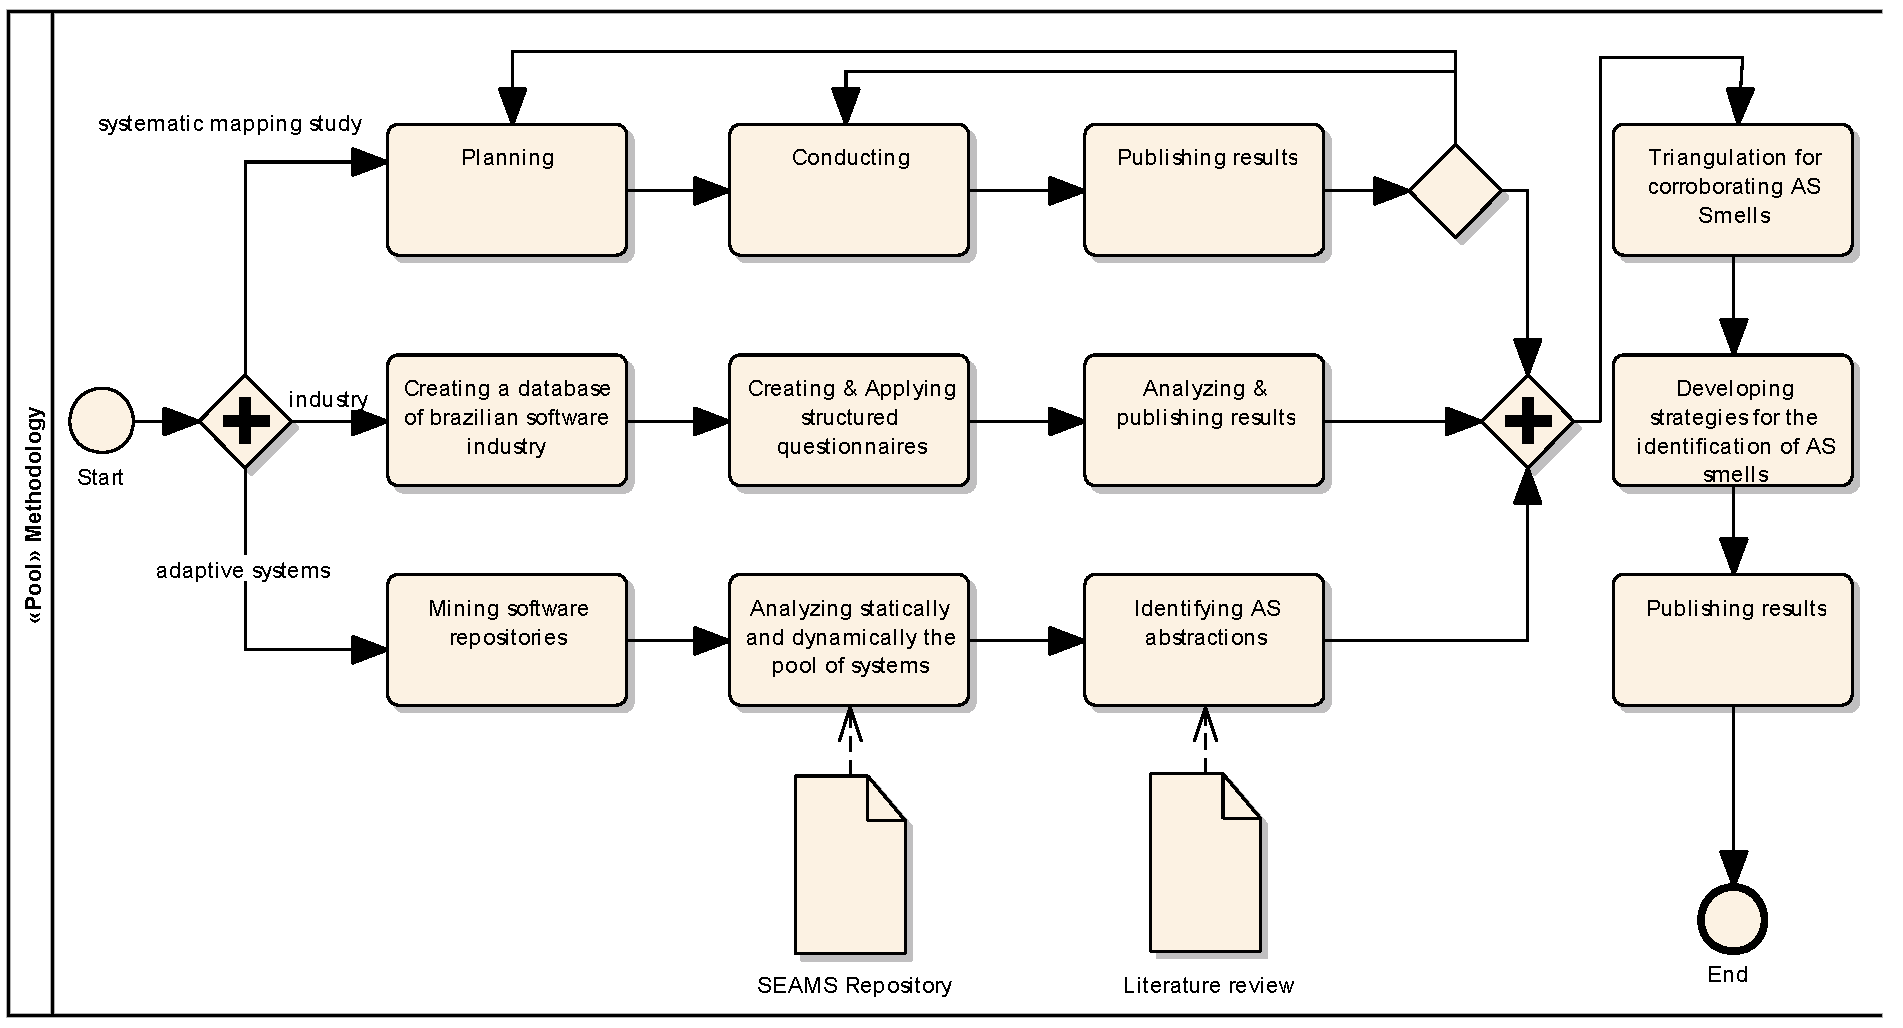
\includegraphics[width=\textwidth]{figures/process.pdf}};

\onslide<1-> {
\node[p] (a) at (4.8,4.8) {};
}

\onslide<2-> {

\node[q] (b) at (4.8,3.5) {};
}

\onslide<3-> {
\node[r] (c) at (4.8,2.2) {};
}
\end{tikzpicture}



\end{frame}


\begin{frame}\frametitle{Evaluation}


\begin{itemize}
	\justifying
	\item Controlled experiments in order to measure the required effort when software engineers need to perform maintenance tasks when there are presence of architectural smells of ASs.
	\vspace{0.5cm}
	\item Precision and recall metrics in order to measure the effectiveness of our set of identification rules for architectural smells of ASs.
	
\end{itemize}

\end{frame}
